\section{Convolutional Network Trained on Synthetic Objects}
\label{sec:simple_cnn}
As a second type of model, we used a simple convolutional neural network (CNN) architecture
consisting of... TODO. To train this CNN, we generated images of artificial 2-D objects
(Fig. \ref{fig:generated_images}) with a variety of different shape, color and texture values. TODO... finish.
Results are shown in Fig. \ref{fig:cnn_results}.

\begin{figure}[h!]
    \begin{center}
        % shape 1
        \begin{subfigure}[b]{0.15\textwidth}
            \begin{center}
                \begin{subfigure}[b]{0.9\textwidth}
                    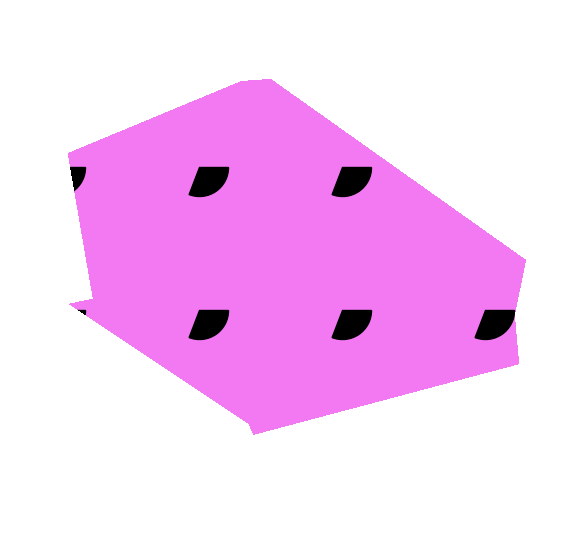
\includegraphics[width=\linewidth]{figures/generated_objects/img0000.png}
                \end{subfigure}
                \begin{subfigure}[b]{0.9\textwidth}
                    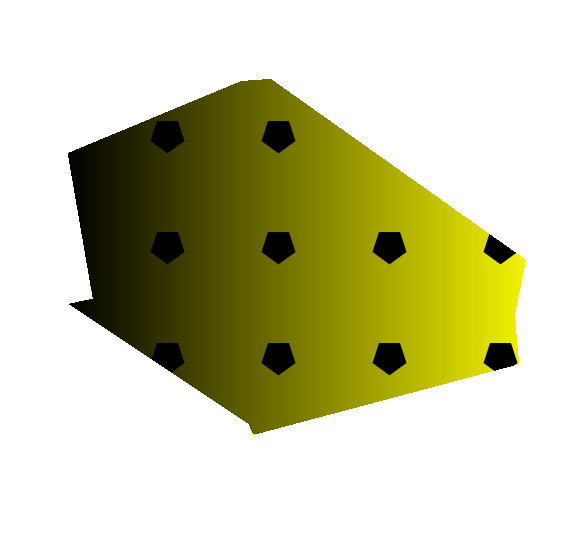
\includegraphics[width=\linewidth]{figures/generated_objects/img0001.png}
                \end{subfigure}
            \end{center}
        \end{subfigure}
        % % shape 2
        \begin{subfigure}[b]{0.15\textwidth}
            \begin{center}
                \begin{subfigure}[b]{0.9\textwidth}
                    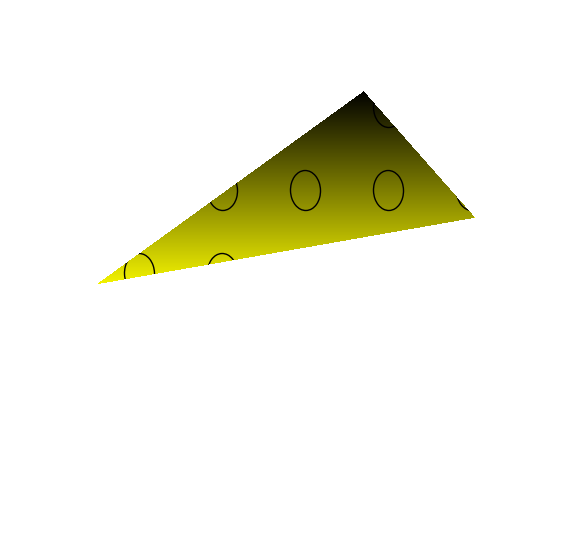
\includegraphics[width=\linewidth]{figures/generated_objects/img0002.png}
                \end{subfigure}
                \begin{subfigure}[b]{0.9\textwidth}
                    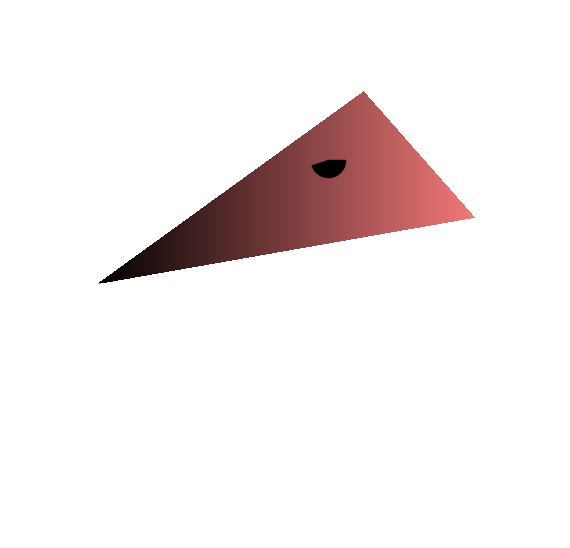
\includegraphics[width=\linewidth]{figures/generated_objects/img0003.png}
                \end{subfigure}
            \end{center}
        \end{subfigure}
        \begin{subfigure}[b]{0.15\textwidth}
            \begin{center}
                \begin{subfigure}[b]{0.9\textwidth}
                    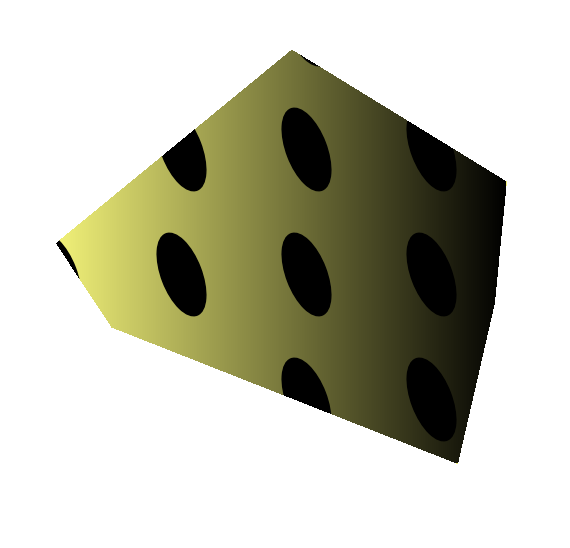
\includegraphics[width=\linewidth]{figures/generated_objects/img0004.png}
                \end{subfigure}
                \begin{subfigure}[b]{0.9\textwidth}
                    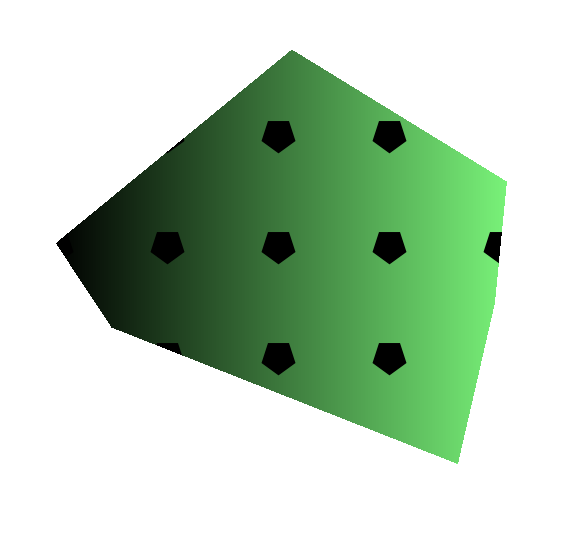
\includegraphics[width=\linewidth]{figures/generated_objects/img0005.png}
                \end{subfigure}
            \end{center}
        \end{subfigure}
    \end{center}
    \caption{Computer-generated images of 2D objects with different shape, color and texture features.}
    \label{fig:generated_images}
\end{figure}

\begin{figure}[h!]
    \begin{center}
        % shape 1
        \begin{subfigure}[b]{0.15\textwidth}
            \begin{center}
                \begin{subfigure}[b]{0.9\textwidth}
                    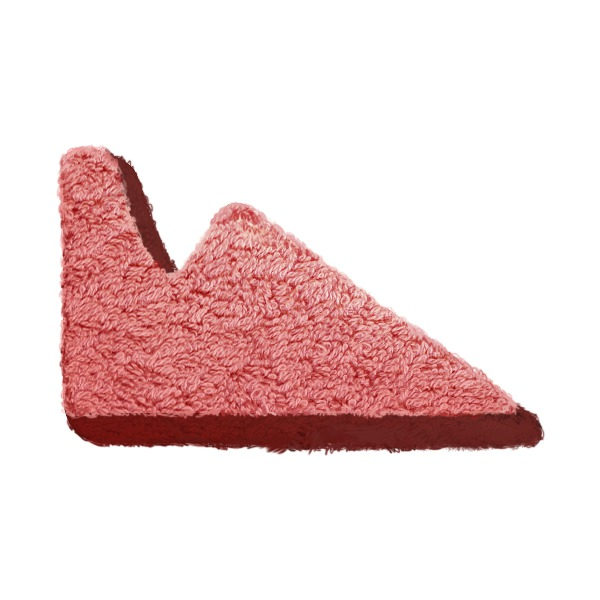
\includegraphics[width=\linewidth]{figures/artist_objects/fake1_carpet_red.jpg}
                \end{subfigure}
                \begin{subfigure}[b]{0.9\textwidth}
                    
\includegraphics[width=\linewidth]{figures/artist_objects/fake1_sponge_yellow.jpg}
                \end{subfigure}
            \end{center}
        \end{subfigure}
        % % shape 2
        \begin{subfigure}[b]{0.15\textwidth}
            \begin{center}
                \begin{subfigure}[b]{0.9\textwidth}
                    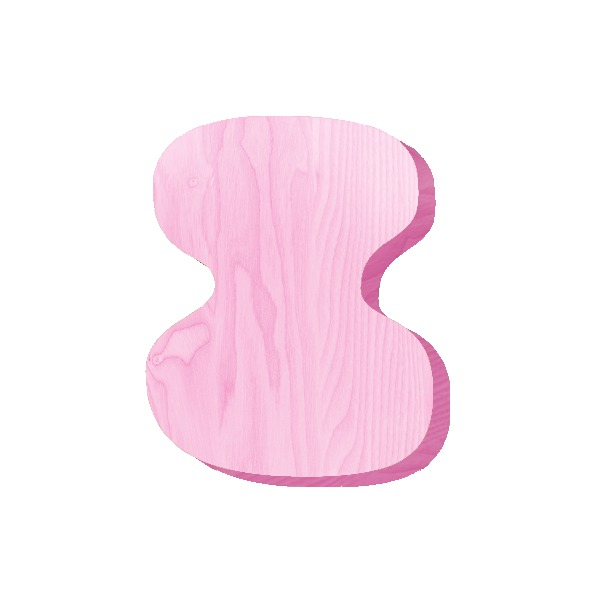
\includegraphics[width=\linewidth]{figures/artist_objects/fake5_wood_pink.jpg}
                \end{subfigure}
                \begin{subfigure}[b]{0.9\textwidth}
                    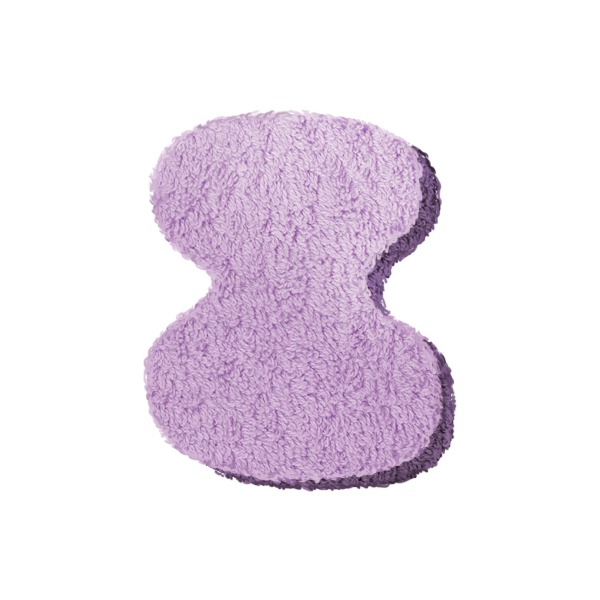
\includegraphics[width=\linewidth]{figures/artist_objects/fake5_carpet_purple.jpg}
                \end{subfigure}
            \end{center}
        \end{subfigure}
        \begin{subfigure}[b]{0.15\textwidth}
            \begin{center}
                \begin{subfigure}[b]{0.9\textwidth}
                    
\includegraphics[width=\linewidth]{figures/artist_objects/fake4_sponge_orange.jpg}
                \end{subfigure}
                \begin{subfigure}[b]{0.9\textwidth}
                    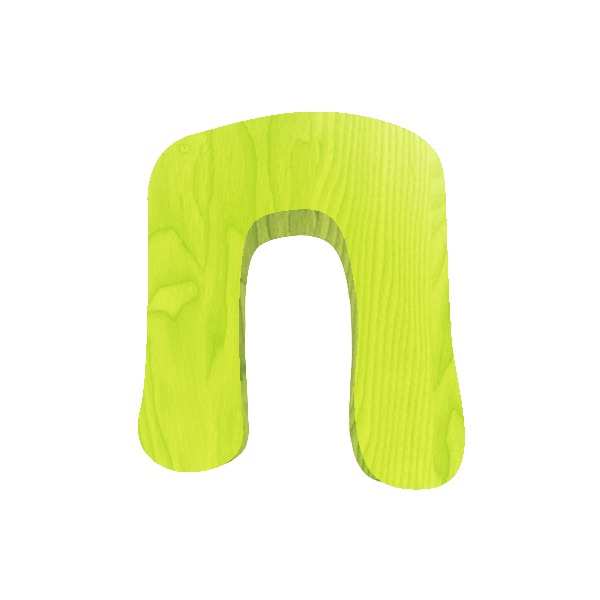
\includegraphics[width=\linewidth]{figures/artist_objects/fake4_wood_green.jpg}
                \end{subfigure}
            \end{center}
        \end{subfigure}
    \end{center}
    \caption{Artist-designed images of 3D objects with different shape, color and texture features.}
    \label{fig:artist_images}
\end{figure}

\begin{figure}[h!]
    \caption{CogPsyc images with different shape, color and texture features (TODO).}
    \label{fig:cogpsyc_images}
\end{figure}

\subsection{Layer-wise Biases}
The first step of our analysis is to evaluate the shape, color and texture biases of VGG-16
at each of its layers, in order to get a picture of how these biases develops along the
higherarchy of the model's internal representation. In order to probe the model, we make
use of two unique image datasets with stimuli that mimic \cite{Smith2002}.

{\bf1. Artist-generated object dataset}: These images were generated by an artist in Adobe
Photoshop. See Fig. \ref{fig:artist_images}.

{\bf2. CogPsyc object dataset}: These images were provided by cognitive psychologist Linda
Smith, and they were used in the experiments of \cite{Ritter2017}. See Fig.
\ref{fig:cogpsyc_images}.

\begin{figure*}[h]
    \begin{center}
        \begin{subfigure}[b]{0.4\textwidth}
            \begin{center}
                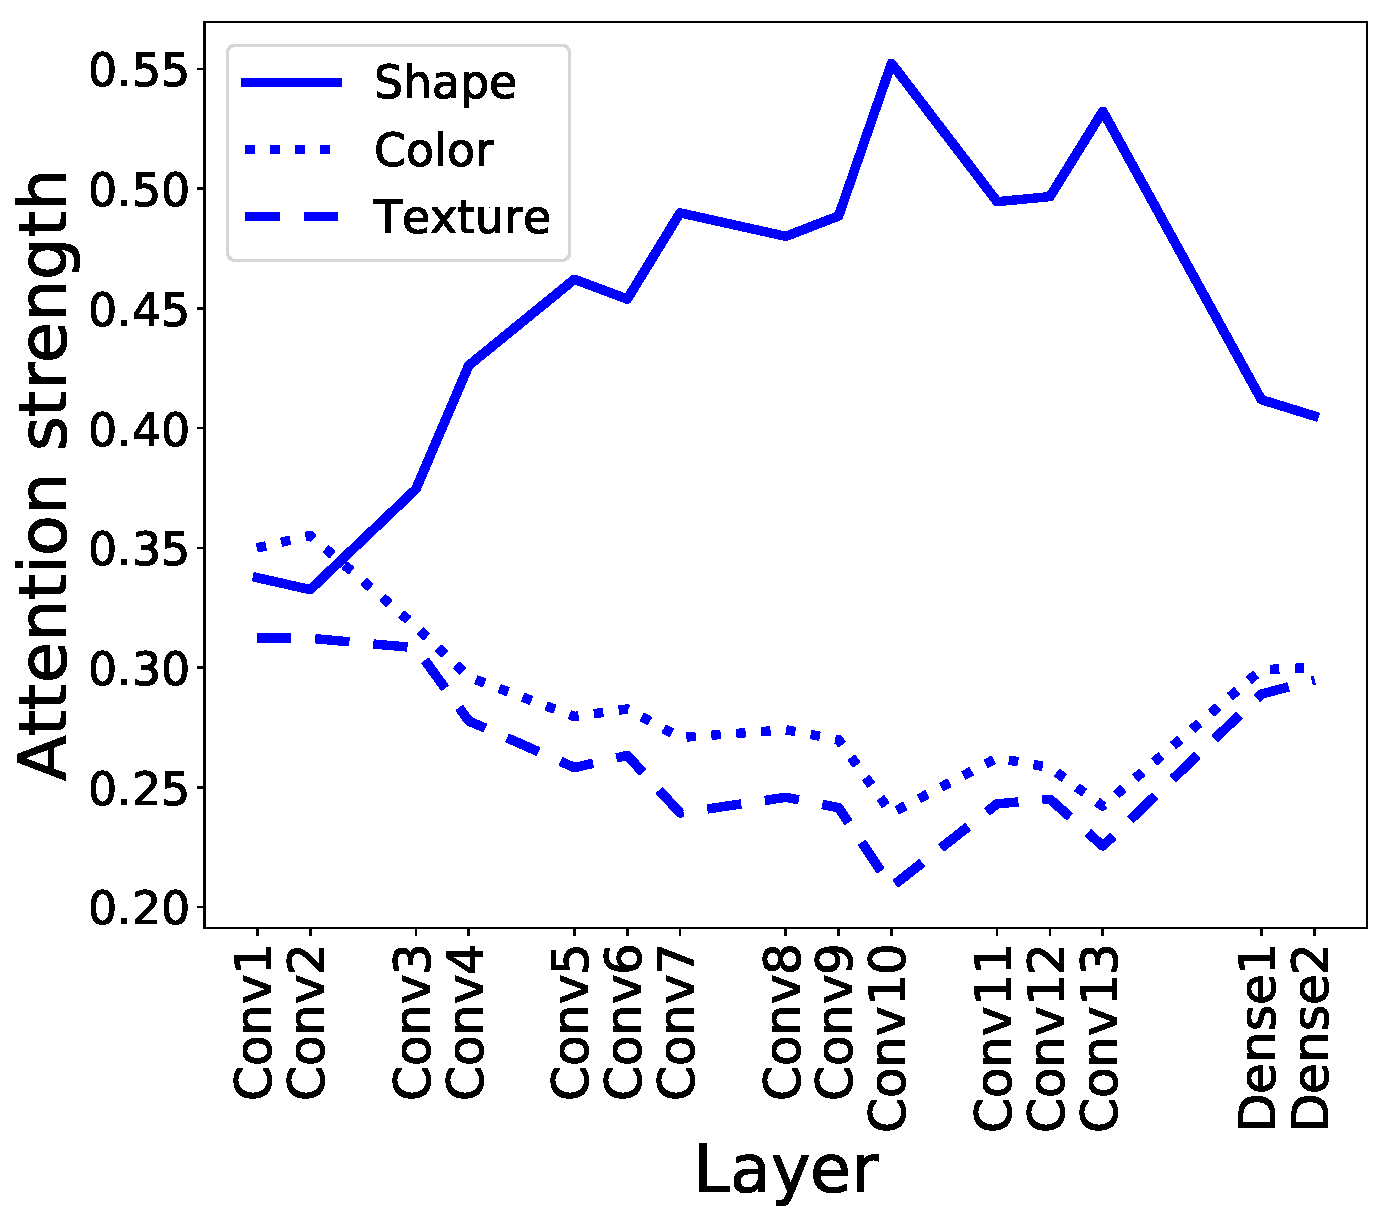
\includegraphics[width=\textwidth]{figures/vgg_layer_biases.pdf}
            \end{center}
            \caption{Artist-generated images}
            \label{fig:biases_artist}
        \end{subfigure}
        \begin{subfigure}[b]{0.4\textwidth}
            \caption{CogPsyc images (TODO)}
        \end{subfigure}
        \caption{VGG-16 layer-wise biases on two image datasets. Attention strength refers to
        the network's similarity score between the target objectand objects that match in
        either shape, color or texture.}
    \end{center}
    \label{fig:layerwise_biases}
\end{figure*}

The layer-wise bias results are shown in Fig. \ref{fig:biases_artist}.

\subsection{Parametric Tests}
The second step of our analysis is to examine how the shape and color biases depend on the intensity
of their respective feature similarities. For these tests, we make use of our computer-generated
images so that we can quantitatively manipulate and evaluate the shape and color features of our
objects. The parametric bias results are shown in Fig. \ref{fig:parametric_others_constant} and
\ref{fig:parametric_others_varying}.
\begin{figure}[h!]
    \begin{center}
        \begin{subfigure}[b]{0.235\textwidth}
            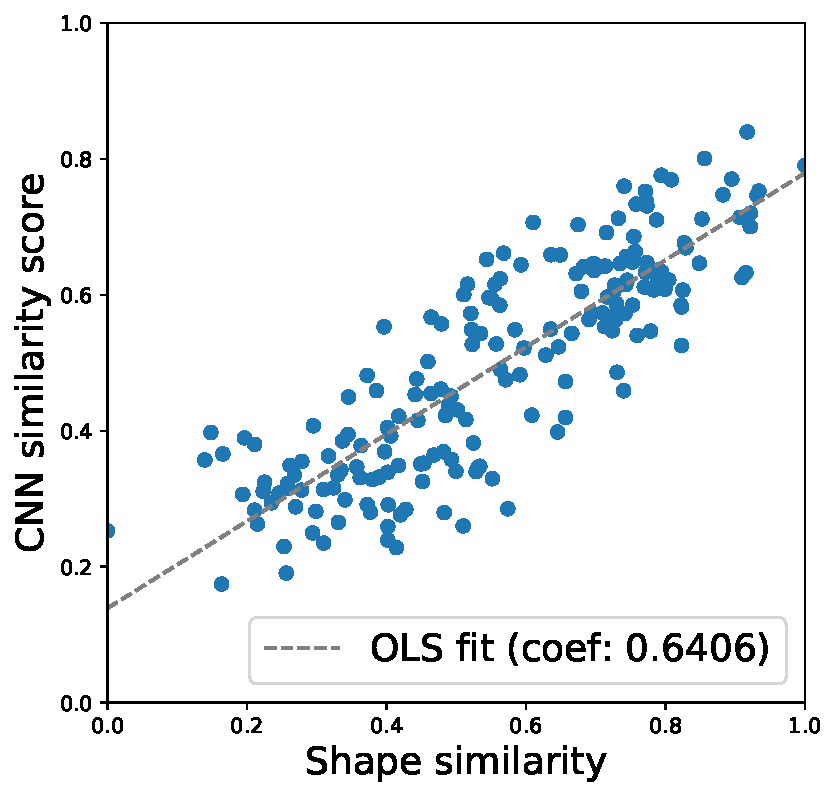
\includegraphics[width=\linewidth]{figures/vgg_shape_parametric_others_constant.pdf}
            \caption{Shape}
        \end{subfigure}
        \begin{subfigure}[b]{0.235\textwidth}
            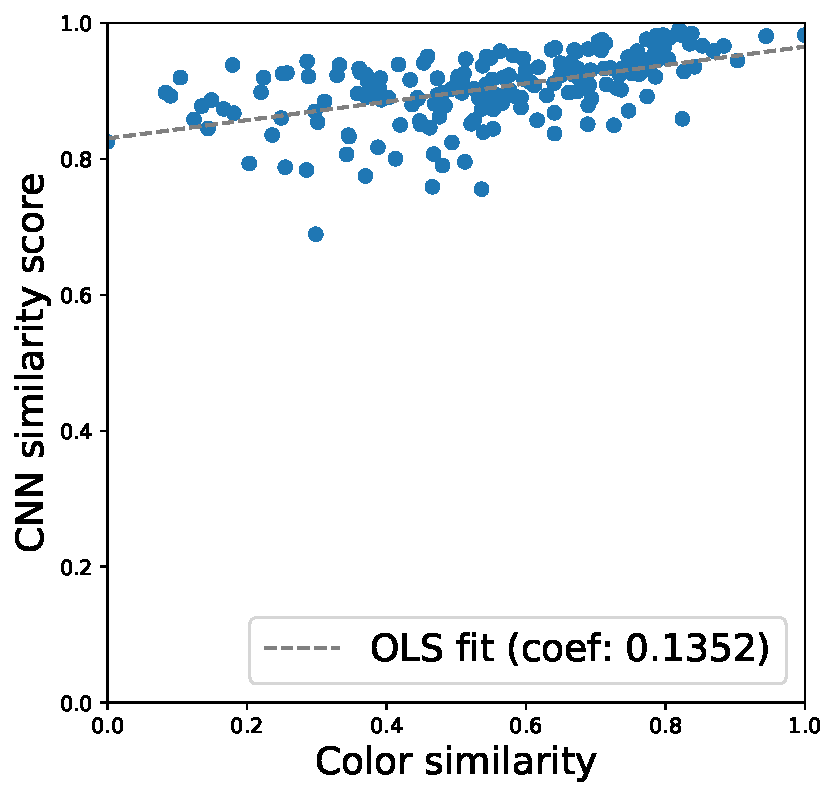
\includegraphics[width=\linewidth]{figures/vgg_color_parametric_others_constant.pdf}
            \caption{Color}
        \end{subfigure}
    \end{center}
    \caption{VGG-16 parametric shape and color biases w/ other features constant.}
    \label{fig:parametric_others_constant}
\end{figure}

\begin{figure}[h!]
    \begin{center}
        \begin{subfigure}[b]{0.235\textwidth}
            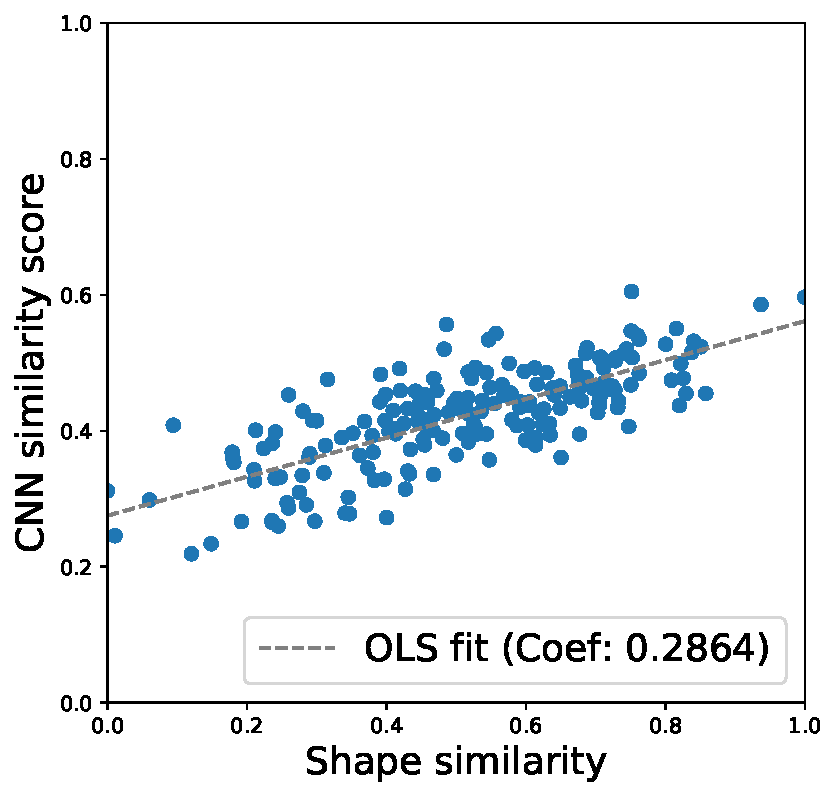
\includegraphics[width=\linewidth]{figures/vgg_shape_parametric.pdf}
            \caption{Shape}
        \end{subfigure}
        \begin{subfigure}[b]{0.235\textwidth}
            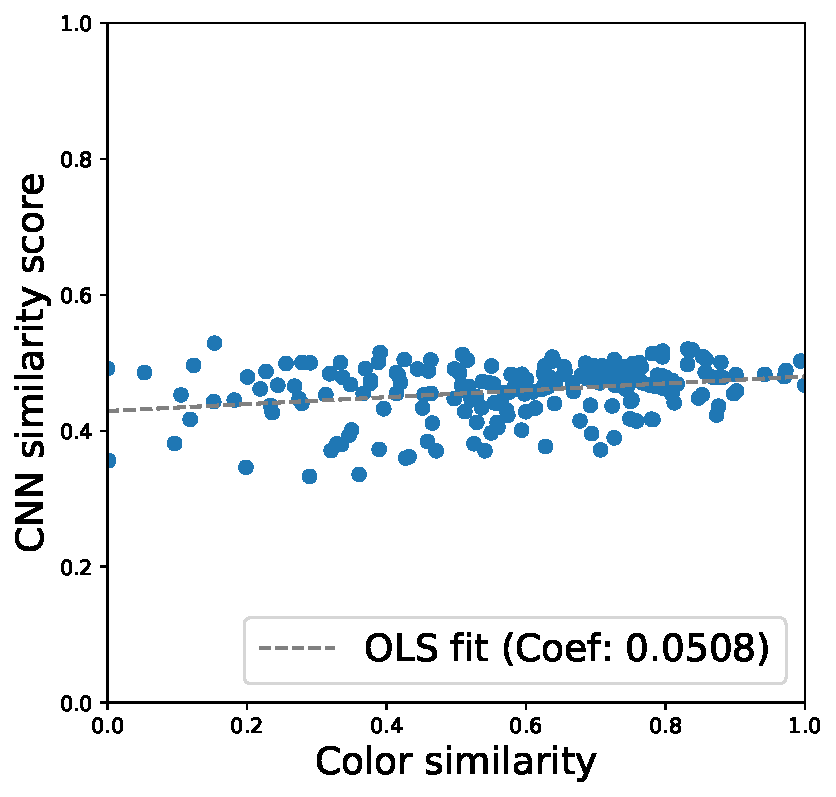
\includegraphics[width=\linewidth]{figures/vgg_color_parametric.pdf}
            \caption{Color}
        \end{subfigure}
    \end{center}
    \caption{VGG-16 parametric shape and color biases w/ other features varying.}
    \label{fig:parametric_others_varying}
\end{figure}